\documentclass[11pt]{article}
\usepackage{../pplmanual}
%%% Commonly Needed packages
\usepackage{graphicx,color,calc}
\usepackage{fancyvrb}
\usepackage{makeidx}
\usepackage{alltt}
\usepackage[linkbordercolor=(0 0 1),citebordercolor=(0 1 0)]{hyperref}
%%\usepackage{xspace} <- creates problems with other hyperlink packages like "html"

%%% Commands for uniform looks of C++, Charm++, and Projections
\newcommand{\CC}{C\hbox{++}}
\newcommand{\emCC}{C\hbox{\em++}}
\newcommand{\charmpp}{\textsc{Charm++}}
\newcommand{\charmc}{\texttt{charmc}}
\newcommand{\projections}{\textsc{Projections}}
\newcommand{\converse}{\textsc{Converse}}
\newcommand{\ampi}{\textsc{AMPI}}
\newcommand{\tempo}{\textsc{TeMPO}}
\newcommand{\irecv}{\textsl{iRecv}}
\newcommand{\sdag}{\textsl{Structured Dagger}}
\newcommand{\jade}{Jade}

%%% Commands to produce margin symbols
\newcommand{\new}{\marginpar{\fbox{\bf$\mathcal{NEW}$}}}
\newcommand{\important}{\marginpar{\fbox{\bf\Huge !}}}
\newcommand{\experimental}{\marginpar{\fbox{\bf\Huge $\beta$}}}

%%% Commands for manual elements
\newcommand{\zap}[1]{ }
\newcommand{\function}[1]{{\noindent{\textsf{#1}}\\}}
\newcommand{\cmd}[1]{{\noindent{\textsf{#1}}\\}}
\newcommand{\args}[1]{\hspace*{2em}{\texttt{#1}}\\}
\newcommand{\prototype}[1]{\vspace{0.2in}\index{#1}}
\newcommand{\param}[1]{{\texttt{#1}}}
\newcommand{\kw}[1]{{\textsf{#1}\index{#1}}}
\newcommand{\uw}[1]{{\textsl{#1}}}
\newcommand{\desc}[1]{\indent{#1}}
\newcommand{\note}[1]{(\textbf{Note:} #1)}
\newcommand{\term}[1]{{\bf #1}\index{#1}}

\makeindex


\makeindex

\title{Charj Manual \\ Compiler Support for Productive Parallel Programming \footnote{last modified 12/14/2012 by Bilge Acun}}
\version{1.0}
\begin{document}

\maketitle

\section{Introduction}

Charj is a new programming language which incorporates syntax, semantic analysis, and optimization targeted at HPC code with its associated compiler. 

\begin{figure}[h]
\begin{center}
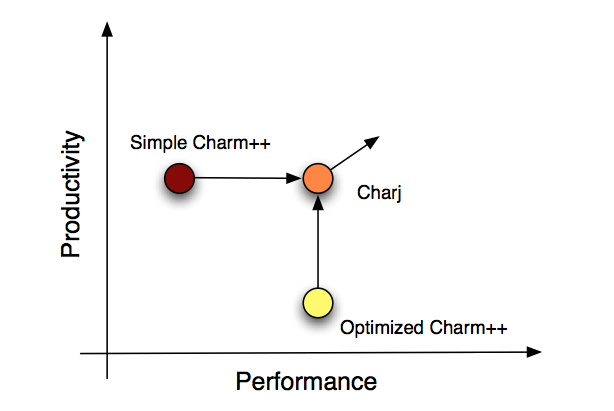
\includegraphics[width=4in]{fig/fig0.png}
\end{center}
\caption{Charj}
\label{fig:fig0}
\end{figure}

With Charj, we aim to allow programmers to achieve the performance associated with carefully written, hand-optimized Charm++ applications, but with much less time and effort. If effect, we hope to combine the productivity that programmers experience when writing relatively simple, naive applications while enjoying performance that would normally require a much greater investment of time, effort, and expertise. 

Charj compiler takes Charj codes as input and produces Charm++ interface (.ci) and C++ code (.C and .h) as an output. 

\begin{figure}[h]
\begin{center}
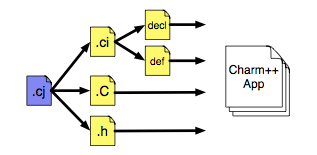
\includegraphics[width=4in]{fig/fig1.png}
\end{center}
\caption{Compilation process for Charj application}
\label{fig:fig1}
\end{figure}

\begin{verbatim}


\end{verbatim}

To make use of Charj;
\begin{enumerate}
\item Build Charm++, then build Charj
\item Write your Charj program
\item Compile and run it!
\end{enumerate}

\section{Building, Compiling and Running}
{\bf To write a program and compile with Charj:}

\begin{enumerate}
\item Go to: {\it charm/src/langs/charj} and {\it "make" } (Assuming Charm++ is already installed)
\item Write your Charj code in a file with {\it .cj} extension. {\it (SampleProgram.cj)}
\item Execute {\it charjc} script on the file {\it SampleProgram.cj}: \\ {\it \$ charm/src/langs/charj/bin/charjc  SampleProgram.cj} \\ \\ For other compiler options, use help: \\ {\it \$ charm/src/langs/bin/charjc -h}

\item After execution of {\it charjc} script, a folder named {\it“SampleProgram.cj.gen”} will be created in the directory of {\it SampleProgram.cj}. This folder will contain the emitted Charm++ files; {\it SampleProgram.ci, SampleProgram.h SampleProgram.cc }.

* Example Charj programs can be found at {\it charm/src/langs/charj/tests}
\end{enumerate}


\section{Writing a Charj Program}

\subsection{General structure of a Charj program; }

\begin{verbatim}

	readonly Main@ mainProxy;	//readonly proxy type
	readonly int value;			//readonly variable
	
	public mainchare Main {
	    public entry Main(CkArgMsg[~]@ m){...} 	//Main constructor
	    public entry void done(){...}		    	//entry method 
	    private int localMethod(int value){...} 	//non-entry method
	}
	public chare_array [1d] SampleChareArray1d{...}	//1d chare array
	public chare_array [2d] SampleChareArray2d{...}	//2d chare array

	public class SampleObject{...}					//sample class

	public chare SampleChare {
	    public entry SampleChare(){...}				//constructor
	    public entry SampleChare(boolean flag){...}	//constructor 2
	    public entry void test(SampleObject obj){...}	//entry method
	}

\end{verbatim}

\subsection{Chare creation and method calls: }

\begin{verbatim}
	SampleChare@ sp = new SampleChare@();
	SampleChareArray1d@ sp1 = new SampleChareArray1d@(x_dim);
	SampleChareArray2d@ sp2 = new SampleChareArray2d@(x_dim, y_dim);
	sp@test();
	sp1@test();
	sp1[index]@test();
	sp2@test(int value);
\end{verbatim}

\subsection{Arrays:}

\begin{verbatim}
	Array<int> foo = new Array<int>([10]);  //1d array of integers of size 10
	foo[i] = ...;
	Array<double, 2> foo2 = new Array<double, 2>([s1, s2]); //2d array of size s1, s2
	foo2[i, j] = ...;
\end{verbatim}

\subsection{SDAG statements:}
These statements can be used inside of any entry method.

\begin{verbatim}
	when receiveMsg(SampleObject obj) {...}

	overlap{	//two overlapping when statements
		when receiveMsg1[i](int iter, SampleObject obj) {...}
		when receiveMsg2[i](int iter, int value) {...}
	}
\end{verbatim}

\subsection{Extern statements: }
If you want to use any other C++ function/feature, you have to define it as {\it extern}.

\begin{verbatim}
	extern atoi;			//define in the beginning of the file
	int x = atoi(y);		//use anywhere
\end{verbatim}

\subsection{Reduction statements:}
Currently only plain reductions are supported.

\begin{verbatim}
	contribute(CkCallback(CkReductionTarget(Main, done), mainProxy));
\end{verbatim}

\subsection{Some Charm++ statements that can be used in a Charj program:}

\begin{verbatim}
	CkExit();
	CkPrintf();
	CkMyPe();
	CkNumPes();
	CkMyNode();
	CkNumNodes();
	CkWallTimer();
	thisProxy
	thisIndex
\end{verbatim}

\end{document}
